\section{Baseline Calibration {\color{YellowGreen} Laurence} }
\label{se:baseline_calibration}

\subsection{Methodology}

The absolute calibration is based on the calibration in $FWHM_0$ beam
described in Sect.~\ref{se:flux_density_equation}. 
Practically, its consists in evaluating a flux
density rescaling factor using a series a OTF scans toward
planets. This flux rescaling factor is an estimate of the
$S_{c}(\nu_{0})$-to-$A_{c}$ ratio of Eq.~\ref{eq:pointsourcephot}. The
calibrator flux density expectation $S_{c}(\nu_{0})$ is obtained as
discussed in Sect.~\ref{se:ref_flux_primaries}, whereas the measured
amplitude $A_c$ is estimated as the average amplitude of the $FWHM_0$
Gaussian fitted from a series of calibrator maps.

Before the flux density estimation, the calibrator raw data are i)
intercalibrated as decribed
in Sect.~\ref{se:intercalibration} and ii) corrected of the
atmospheric attenuation as described in Chapter~\ref{se:opacities}. To
refine the intercalibration between the two $1$-mm arrays after the
KID Hertz to Jy/beam conversion factor estimates, a flux rescaling
factor per array is calculated. Regarding the correction of the
atmospheric attenuation, we
resort to the 'corrected skydip' opacity correction, as described in
Sect.~\ref{se:corrected-skydip}, for the baseline calibration.
However, calibrations relying on the
'taumeter' (Sect.~\ref{se:taumeter-method}) and the 'skydip'
(Sect.~\ref{se:skydip-method}) methods are also derived, and will be
used for performing the photometry robustness tests discussed in
Sect.~\ref{se:photometry_others}. Finally, the telescope-driven beam
effect, discussed in Sect.~\ref{se:obsdate_variations}, is mitigated by
using the baseline scan selection of
Sect.~\ref{se:data_selection}, in which, we recall, the most
impacted scans are discarded by mean of a cut on the observation
date. 

%When available, the prefered primary calibrator is Uranus,
%which allies a strong flux density and a small extention. At the IRAM
%$30$-m telescope, the apparent Uranus disc diameter varies from
%$3.3''$ to $3.7''$. In Sect.~\ref{se:ref_flux_uranus_neptune}, Uranus
%disc is accounted for in evaluating the flux density
%expectation.
%To retrieve the
%flux density of a point source after absolute calibration using
%Uranus, a correction has also to be applied to account for the
%beam widening effect of Uranus disc. The response of the $FWHM_0$
%Gaussian amplitude estimator (as of
%Eq.~\ref{eq:fixed-width-gaussian-estimator})
%of a map of Uranus disc
%slightly differs from the one of a point-like source. In
%Sect.~\ref{se:photometric_correction}, we find that the $\sigma_0$
%Gaussian amplitude estimate
%of the map of a point source varies as
%$(2\sigma_0^2)/(\sigma^2 + \sigma_0^2)$, where $\sigma$ is the main
%beam width. The convolution of Uranus disc and the $\sigma$-width
%Gaussian widens the main beam size to $\sigma_{\rm{u}}$. Thus, the
%absolute calibration factor evaluated on Uranus has to be corrected
%from the Uranus widening factor:
%\begin{equation}
%  C_{u} = \frac{\sigma^2 + \sigma_0^2}{\sigma_{\rm{u}}^2 + \sigma_0^2} 
%\end{equation}
%to retrieve point-source flux densities. Using the main beam FWHM of
%$11.2''$ at $1$mm and $17.4''$ at $2$mm, as reported in Sect.~\ref{se:MB},
%the beam widening is of $0.2''$ at $1$mm and $0.13''$ at $2$mm and the
%widening factors are $0.985$ and $0.994$ at 1 and 2 mm respectively.

 
\subsection{Scan selection}

To illustrate the baseline selection efficiency, we present Uranus
measured-to-predicted flux density ratios as a fonction of the 2D
Gaussian FWHM estimates and color-coded from the observation dates
given in UT hours in the first panels of
Fig.~\ref{fig:calib_uranus_vs_fwhm_all}
We note that the flux density estimates have been corrected by the
rescaling factors, so that the flux density ratios are equal to unity
in average by contruct. First row panels of
Fig.~\ref{fig:calib_uranus_vs_fwhm_all} show the flux ratio after
correction from the baseline rescaling factors, whereas second and
third row panels are for 'taumeter'-based and 'skydip'-based absolute
calibration respectively. For the baseline calibration, the selected
scan flux ratios (shown as full circles) are stable against the beam
FWHM. The 'taumeter'-based selected flux ratios show more dispersion
but no significant dependence on the FWHM. The flux ratio-to-FWHM
correlation is most clearly seen for the 'skydip'-based calibration:
broaden beams are associated with lower fluxes. However, this
correlation is efficiently mitigated after the baseline scan
selection. The residual anti-correlation between
the 'skydip' flux ratios and beams originates from a mild
correlation of the flux density with the atmospheric transmission as
discussed later in Sect.~\ref{se:photometry_others}. 

The Uranus available scan numbers and the scan numbers after the baseline scan
selection was performed are given per observation campaigns and for
the combination of the three considered campaigns in
Table~\ref{tab:absolute_calibration_scan_numbers}. For N2R9 and N2R14,
which were both February campaigns one year apart, Uranus was mainly
visible during the day. As a results, only two good scans are used to
derive the absolute calibration. However, we will verify in
Sect.~\ref{se:photometry_baseline} that this suffices to obtain an
accurate photometry. By contrast, due to the night time visibility of
Uranus during N2R12, almost all the available scans meet the baseline
section criteria. 


% ALL METHOD RESULTS 
\begin{table}[th]
\begin{center}
\begin{tabular}{|c|c|c|c|c|c|}
  \hline
  \multicolumn{2}{|c|}{}            &  \multicolumn{4}{|c|}{Datasets} \\\cline{3-6}
  \multicolumn{2}{|c|}{Scan number} &  N2R9  & N2R12  &  N2R14  &  Combined \\
  \hline\hline
  \multicolumn{2}{|c|}{Total}       &   27   &   25    &   40    &    92  \\
  \hline
  Selected & Baseline               &   2    &   22    &    2    &    26  \\
           & Photocorr              &   2    &   24    &   12    &    38  \\
\hline\hline
\end{tabular}
\caption[Absolute calibration scan numbers]{Number of scans for the absolute calibration}
\label{tab:absolute_calibration_scan_numbers}
\end{center}
\end{table}


%%%%%%%%%%%%%%%%%%%%%%%%%%%%%%%%%%%%%%%%%%%%%%%%%%%%%%%%%%%%%%%%%%%
%    Flux ratio vs FWHM

\begin{figure}[ht!]
  \begin{center}
    % corrected skydip
    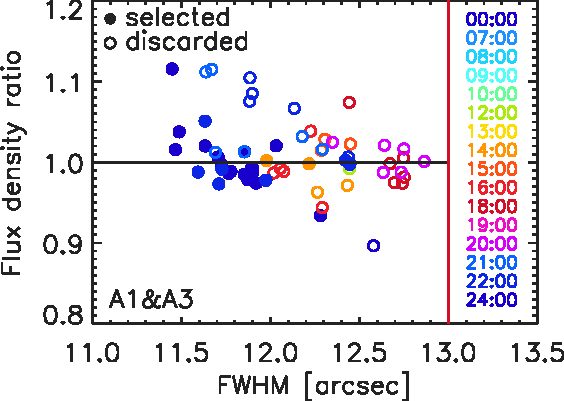
\includegraphics[clip=true, trim={0, -0.3cm, -0.3cm, 0}, width=0.35\textwidth]{Figures/Calibration/plot_flux_density_ratio_fwhm_uranus_corrected_skydip_narrow_1mm.pdf}
    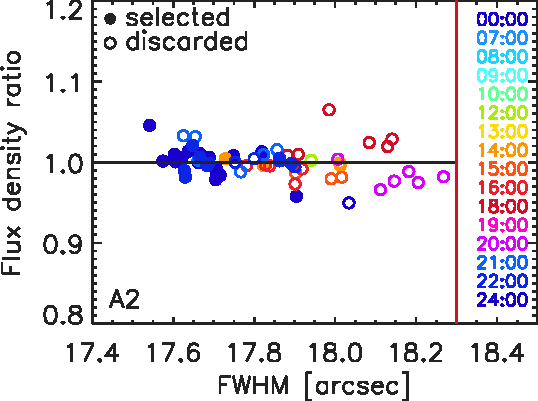
\includegraphics[clip=true, trim={0, -0.3cm, -0.3cm, 0}, width=0.3337\textwidth]{Figures/Calibration/plot_flux_density_ratio_fwhm_uranus_corrected_skydip_narrow_a2.pdf}
    % taumeter
    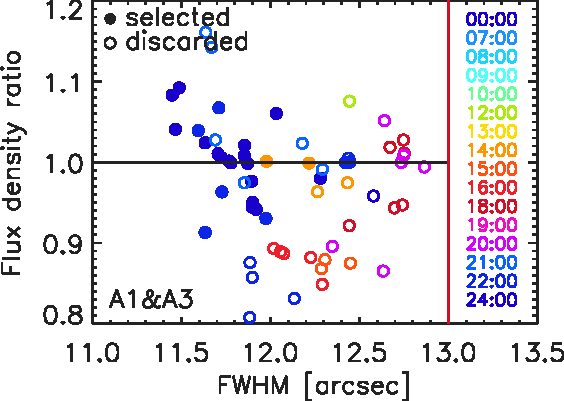
\includegraphics[clip=true, trim={0, -0.3cm, -0.3cm, 0}, width=0.35\textwidth]{Figures/Calibration/plot_flux_density_ratio_fwhm_uranus_tau225_narrow_1mm.pdf}
    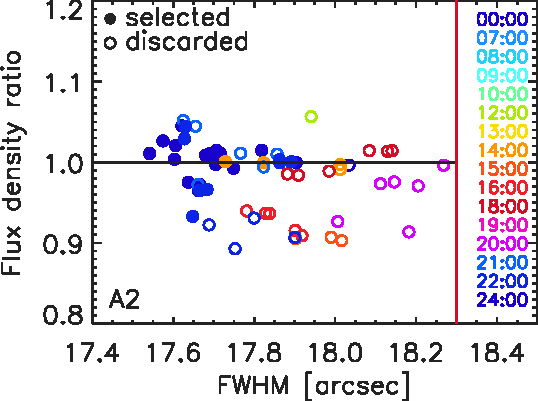
\includegraphics[clip=true, trim={0, -0.3cm, -0.3cm, 0}, width=0.3337\textwidth]{Figures/Calibration/plot_flux_density_ratio_fwhm_uranus_tau225_narrow_a2.pdf}
    % skydip
    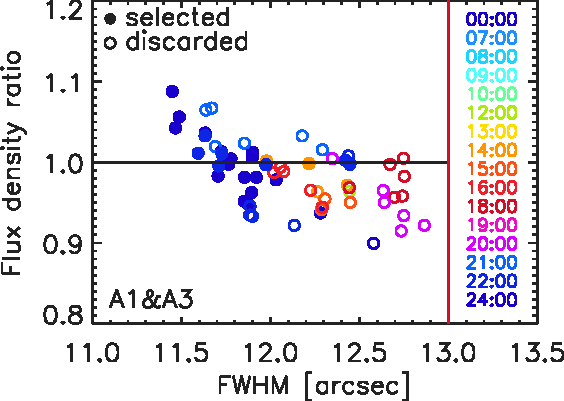
\includegraphics[clip=true, trim={0, -0.3cm, -0.3cm, 0}, width=0.35\textwidth]{Figures/Calibration/plot_flux_density_ratio_fwhm_uranus_skydip_narrow_1mm.pdf}
    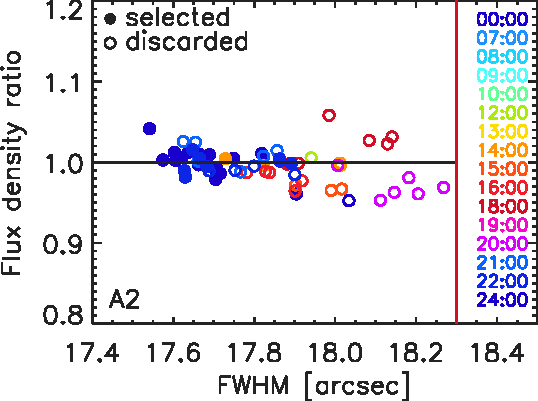
\includegraphics[clip=true, trim={0, -0.3cm, -0.3cm, 0}, width=0.3337\textwidth]{Figures/Calibration/plot_flux_density_ratio_fwhm_uranus_skydip_narrow_a2.pdf}
    % corr. sky. photocorr demo
    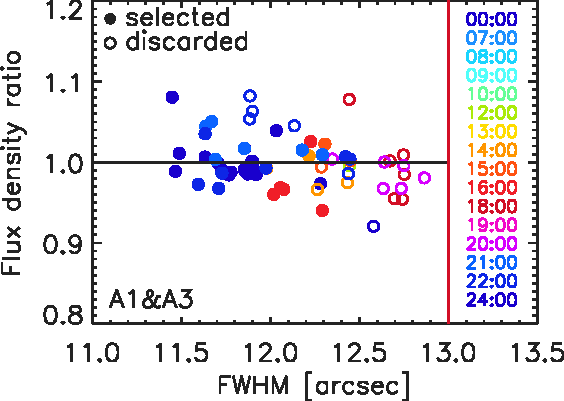
\includegraphics[clip=true, trim={0, -0.3cm, -0.3cm, 0}, width=0.35\textwidth]{Figures/Calibration/plot_flux_density_ratio_fwhm_uranus_corrected_skydip_photocorr_demo_narrow_1mm.pdf}
    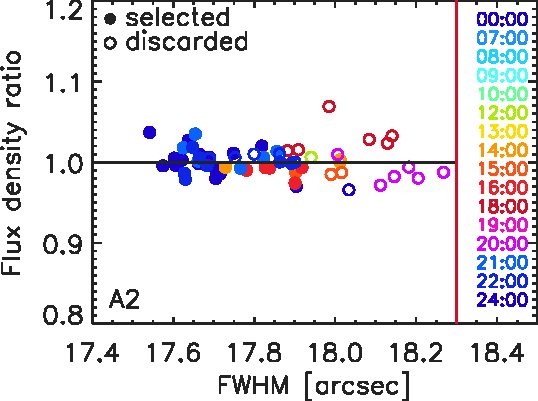
\includegraphics[clip=true, trim={0, -0.3cm, -0.3cm, 0}, width=0.3337\textwidth]{Figures/Calibration/plot_flux_density_ratio_fwhm_uranus_corrected_skydip_photocorr_demo_narrow_a2.pdf}
    % corr. sky. photocorr pointing
    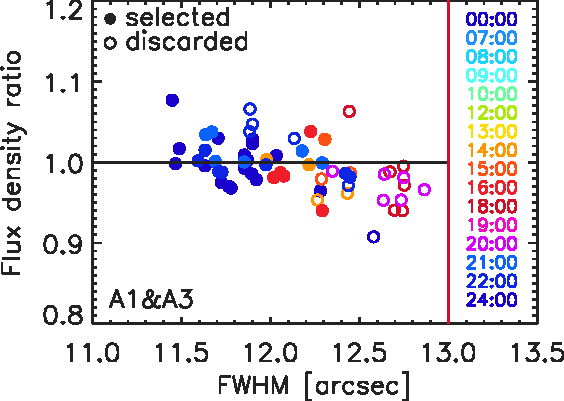
\includegraphics[clip=true, trim={0, -0.3cm, -0.3cm, 0}, width=0.35\textwidth]{Figures/Calibration/plot_flux_density_ratio_fwhm_uranus_corrected_skydip_photocorr_pointing_narrow_1mm.pdf}
    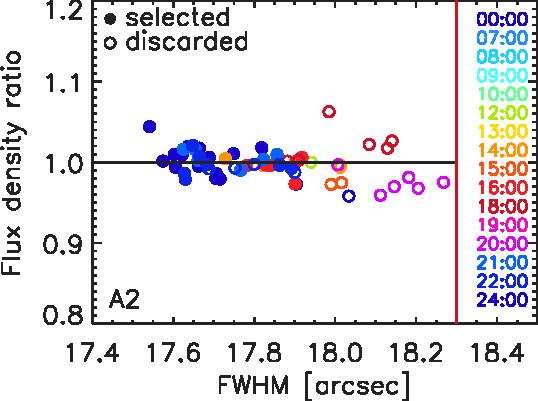
\includegraphics[clip=true, trim={0, -0.3cm, -0.3cm, 0}, width=0.3337\textwidth]{Figures/Calibration/plot_flux_density_ratio_fwhm_uranus_corrected_skydip_photocorr_pointing_narrow_a2.pdf}
    \caption[Uranus flux density stability against FWHM]{
      Uranus flux density ratio vs beam size for five
      calibration methods. The ratio of 
      Uranus measured flux densities to expectations in fonction of the
      measured 2D Gaussian beam FWHM is shown for the $1$-mm array
      combination (left column) and for array 2 (right column) after absolute
      calibration using (\emph{first row}:) the baseline method, as
      well as (\emph{second row}:) the 'taumeter'-based and
      (\emph{third row}:) the 'skydip'-based methods, and methods
      relying to (\emph{fourth row}:) the 'demo' and (\emph{fifth
        row}:) the 'pointing' photometric corrections. These plots
      include all Uranus scans acquired during N2R9, N2R12 and N2R14
      campaigns and whose beam FWHM are below the threshold indicated
      by the vertical red lines, (open circles), as
      well as the scans that met the baseline selection criteria (filled
      circles).}
\label{fig:calib_uranus_vs_fwhm_all}
\end{center}
\end{figure}


\subsection{Stability against the atmospheric transmission}

We test the stability of Uranus flux density ratio
against the atmospheric transmission. The later quantity, we
recall, depends on the measured zenith opacity $\tau$ and the scan
average airmass $x = $cosec$(\delta)$ as $\exp{-\tau \cdot x}$. In
Fig.~\ref{fig:uranus_flux_obstau}, Uranus flux ratios of Array 1,
Array 3, the $1$-mm array combination and Array 2 are plotted as a
function of the atmospheric transmission for the three considered
observation campaigns (N2R9, N2R12 $\&$ N2R14). Although Uranus flux
ratio per campaign is equal to the unity in average, any trend as
a fonction of the observing conditions would sign the presence of a
systematic effect. However, no sizable dependencies of the flux ratio
on the atmospheric transmission is observed. This constitutes a first
indication of the robustness of the flux density estimates againts the
atmospheric conditions using the baseline calibration. This will be
further tested using more scans in Sect.~\ref{se:photometry_baseline}.   


\begin{figure}[ht!]
  \begin{center}
    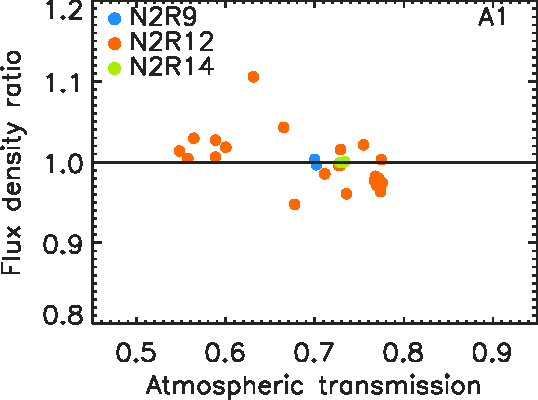
\includegraphics[clip=true, trim={0, -0.3cm, -0.3cm, 0}, width=0.35\textwidth]{Figures/Calibration/plot_flux_density_ratio_obstau_uranus_corrected_skydip_narrow_a1.pdf}
    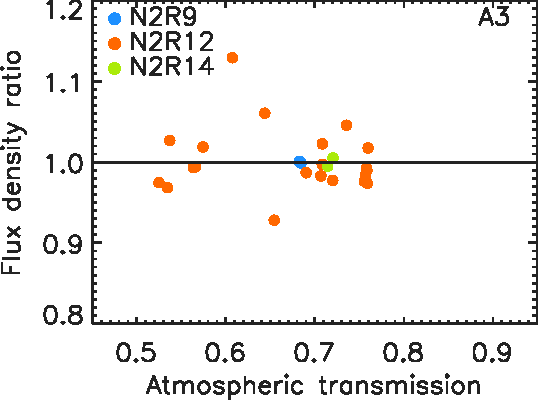
\includegraphics[clip=true, trim={0, -0.3cm, -0.3cm, 0}, width=0.35\textwidth]{Figures/Calibration/plot_flux_density_ratio_obstau_uranus_corrected_skydip_narrow_a3.pdf}
    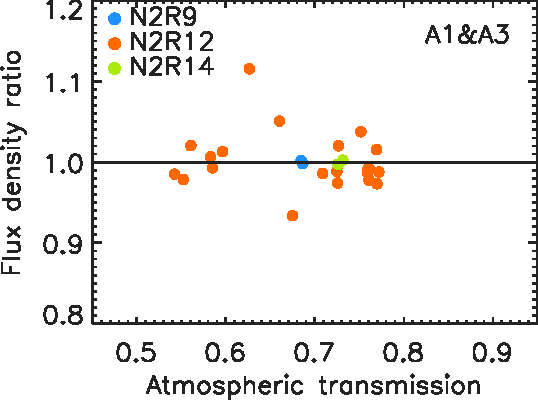
\includegraphics[clip=true, trim={0, -0.3cm, -0.3cm, 0}, width=0.35\textwidth]{Figures/Calibration/plot_flux_density_ratio_obstau_uranus_corrected_skydip_narrow_1mm.pdf}
    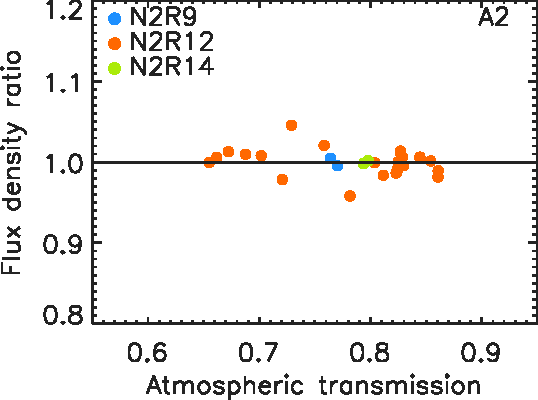
\includegraphics[clip=true, trim={0, -0.3cm, -0.3cm, 0}, width=0.35\textwidth]{Figures/Calibration/plot_flux_density_ratio_obstau_uranus_corrected_skydip_narrow_a2.pdf}
    \caption[Uranus flux density stability against atmospheric
      transmission]{Uranus flux density ratio stability against the
      atmospheric transmission using the baseline calibration.
      The measured-to-modeled flux density
      ratio as a fonction of the measured atmospheric transmission is
      shown for array 1 (upper left), array 3 (upper right), 1mm array
      combination (lower left) and array 2 (lower right).
      The datapoints denote the flux ratio of Uranus scans acquired
      during N2R9 in blue, N2R12 in orange and N2R14 in chartreuse
      (yellow green).
      For each campaign, flux ratios are equal to unity in average by
      construction. We observe no sizable systematic effect depending
      on the atmospheric transmission, modelled as the decreasing exponential
      function of the zenith opacity times the air mass at the
      telescope elevation.}
\label{fig:uranus_flux_obstau}
\end{center}
\end{figure}


\subsection{Comparison with other opacity correction methods}

Whereas the baseline calibration relies on correcting for the
atmospheric attenuation using the 'corrected skydip' method described
in Sect.~\ref{se:corrected-skydip}, here we derive the absolute
calibration factor using the 'taumeter' and the 'skydip' opacity
correction methods, as discussed in Sect.~\ref{se:taumeter-method} and
Sect.~\ref{se:skydip-method}. The baseline Uranus measured-to-modeled
flux ratio as a function of the atmospheric transmission for A1$\&$A3
and for A2 are copied in the first row of
Fig.~\ref{fig:calib_uranus_vs_atmtrans_all}, and are
compared to the 'taumeter'-based flux ratios (second row) and
'skydip'-based flux ratios (third row). We observe more dispersion for
the 'taumeter'-based flux ratio, whereas the 'skydip'-based ratios are
very similar as the 'baseline' ratios except for a slight decrease of
the flux at low atmospheric transmission. We further quantify the
difference between methods in evalutating i) the average absolute
calibration rescaling factor with respect to the baseline factor and
ii) the rms dispersion of the measured-to-modeled flux ratio. These
quantities are gathered in Table~\ref{tab:Abs_calibration_results_all}
in the rows labeled 'Factor' and 'RMS' respectively. Resorting to a
different opacity correction results in small changes of the absolute
calibration factors, up to a $13\%$ increase for Array 1 using
'skydip'. However, these modifications of the absolute calibration has
no sizable impact on the photometry, as we will check in
Chapter~\ref{se:photometry} (see
e.g. Table~\ref{tab:Calibration_results_all}). From the RMS row, we
confirm an increase of the 'taumeter'-based flux ratio dispersion of
about $40\%$ at 1 mm and about $60\%$ at 2mm w.r.t. the baseline
dispersion, whereas 'skydip' dispersions are basically the same as
'baseline'. Thus the 'taumeter' and 'skydip' methods can be used for
the absolute calibration in complement to the baseline method, e.g. to
perform robustness tests as in Chapter~\ref{se:photometry}.  

  

